\documentclass{article}
%\documentclass{river-journal}
%\usepackage{rivps}
%\usepackage[mtbold]{mathtime}

\usepackage{graphicx}
\usepackage{graphics}
%\usepackage{subfigure}
\usepackage{cite}
\usepackage{url}
\usepackage{subcaption}
\usepackage{multirow}

%Common packages.
\usepackage{cite}
\usepackage{amsmath}
\usepackage{amssymb}
\usepackage{graphicx}
\usepackage{listings}
\usepackage{url}
\usepackage{appendix}
\usepackage{adjustbox}
\usepackage{subcaption}
\usepackage{amsthm}
\usepackage{ltxtable}
\usepackage{rotating}

%NOT TO BE INCLUDED IN SUBMISSION.
\usepackage{hyperref}

%Need to be at last.
\usepackage{cleveref}


% for alternatives, see appendix of manual

%\newtheorem{guess}{Conjecture}

% bibliographies
\bibliographystyle{plain}
% also tested with natbib



\title{Exploring Potential 6LoWPAN Traffic Side Channels}
\author{Yan Yan \and Elisabeth Oswald \and Theo Tryfonas}

\begin{document}
\maketitle
%\begin{opening}
%\institute{University of Bristol,  \texttt{y.yan@bristol.ac.uk}}
%\end{opening}

%\runningtitle{Exploring Potential 6LoWPAN Traffic Side Channels}
%\runningauthor{Y. Yan}

\subsection*{Abstract}
The Internet of Things has become a reality: small connected devices feature in everyday objects
including childrens' toys, TVs, fridges, heating control units, etc. Supply chains feature sensors
throughout, and significant investments go into researching next-generation healthcare, 
where sensors monitor wellbeing. A future in which sensors and other (small) devices interact to create sophisticated applications seems just around the corner . All of these applications have a fundamental need for security and privacy and thus we need to deploy cryptography as part an attempt to secure them. In this paper we explore a particular type of flaw, namely side channel information, on the protocol level. Our research investigates the potential for utilising packet length and timing information (both are easily obtained) to extract interesting information from a system, despite the use of cryptography. 

%\keywords{6LoWPAN, Side Channels, Traffic Analysis}

\section{Introduction}
The expression `Internet of Things' (IoT) can refer to a multitude of objects and protocols, which share that they have been purposefully designed for resource constraint environments. Whereas the typical TCP/IP network stack produces considerable overhead to achieve quality of service for applications that are based on it, the nature of many IoT `things' is such that a full implementation of it would not be practical. Often `things' are sensor, which are devices that have to function on little resources (most importantly power). Thus a whole host of new networking protocols have been developed over the years to cater for such resource constrained devices: 6LoWPAN is the `tiny' version of IPv6, UDP tends to be used instead of TCP/IP, DTLS can be used for end-to-end security or one can directly invoke 802.15.4 Security which is part of 6LoWPAN, and finally CoAP(s) is the replacement for HTTP(s). Thus there are two options (802.15.4, and DTLS) to secure communications between the `things' and a server/gateway. 

Implementing cryptography correctly and securely has proven to be a massive challenge as evidenced by the multitude of implementation attacks over the years. Triggered off by research that showed how to utilise additional information via timing and power side channels\cite{DPA}, many different flavours of side channel attacks were discovered over the last decade. Many attacks use phyiscal information (such as low level execution timings or power consumption) to recover secret keys, but many other attacks use protocol level information (such as packet lengths, types of packets or protocol messages) to recover information about plaintexts, devices in the network, or the network itself. 
There exists a considerable body of work in the context of conventional, i.e. HTTPs over TCP/IP network, but the applicability of (some) of these attacks in the context of a typical IoT protocol stack is lacking. This is the gap that we would like to address within this submission. 

This paper is structured as follows: after reviewing some relevant attack paths for HTTPs over TCP/IP in the following subsection, we provide a brief introduction to the necessary protocol and network features in \Cref{sec: IotProtocols}.  We discuss the impact of packet length leakage in \Cref{sec: PacketLen}, followed by an analysis of the response time leakage in \Cref{sec: ResponseTime}. We summarise our work in \Cref{sec: Conclusion}. 

\subsection{Related Work\label{subsec: RelatedWork}}
%Write about attacks that exploit packet length and response times in the context of TCP/IP. Reflect on web applications and how the same might happen if more interesting applications might be deployed that involve IoT objects.

%Literatures about Traffic Analysis...
Traffic Analysis is well studied in the context of encrypted Internet traffic, especially for web applications based on HTTPs and TCP/IP. The landmark study by Chen et al. \cite{WebSidechannel} discussed different side channel attacks against web applications and \cite{SuggestBox} studied the practicability of an attack specifically targeted Google and Bing search boxes. Later work by Mather and Oswald \cite{PinpointWeb} proposed the use of Mutual Information to pinpoint the potential leakage points in web traffic. For non-HTTPs applications, the papers \cite{AppleMsg}, \cite{Language} and \cite{VideoTraffic} described attacks against encrypted text, voice and video traffic respectively. Machine learning is widely used to analyse the traffic, and behaviours of different classifiers are studied by \cite{HClassifier} and \cite{Peekaboo}. Based on all these published works we can conclude that two features, the packet length and response time, are the most exploited ones among all attacks. Different countermeasures were studied by \cite{TrafficMorphing}, \cite{HTTPOS} and \cite{FTE}.

Reflecting on IoT applications, we stipulate that most of these attacks may still be applicable, as we intend to demonstrate in this paper. Considering the future vision that IoT devices could be indeed connected to the Internet with even more sensitive data flowing over different networks, the task of designing secure IoT applications becomes increasingly challenging.

%Literatures about 6LoWPAN security
With regard to the aspect of protocol design, the recent paper \cite{6LoWPANAtk} summarised some known flaws of 6LoWPAN, including its susceptibility to the Fragmentation Attack\cite{FragAtk}, Sinkhole Attack\cite{Sinkhole}, Hello Flood Attack\cite{HelloFlood}, Wormhole Attack\cite{Wormhole} and Blackhole Attack\cite{Blackhole}. In addition, \cite{802154SecIssues} reported certain problematic designs in 802.15.4 security\cite{802154}. However we do not discuss further about these designing flaws as they lay into a different aspect of the security issues addressed by this paper.

%\textbf{TODO: if space and time say some more about these attacks. At least say if they relate to the type of leakage we are exploiting or if they are completely independent (which is what I would guess). }

\section{A Typical IoT Protocol Stack\label{sec: IotProtocols}} 
%A typical sensor network is built as described in \ref{Protocols}.
%IoT Protocols
Many protocols are proposed for different IoT applications adapting to various requirements. For example, some smart houses simply use WiFi for connectivity and VANETs\footnote{Vehicular ad hoc networks} may adopt DSRC\cite{DSRC}. 

%WSN Protocols
In this paper we focused on 6LoWPAN\cite{rfc4944} which is based on 802.15.4\cite{802154}. These standards are designated for constrained environments such as Wireless Sensor Networks,  but other competing standards exist at different layers. Bluetooth Low Energy(BLE)\cite{BLE} is a strong competitor to 802.15.4 as well as the LiFi\cite{LiFi} technology. Zigbee\cite{Zigbee} is originally intended as a collective protocol over 802.15.4 but it has been recently adapted to IP-based network in ZigbeeIP\cite{ZigbeeIp} so to compete with 6LoWPAN. The RIME stack\cite{RIME} proposed a set of non-layered primitives over 802.15.4 but it is likely to be phased-out probably due to the reluctance of interoperability with the TCP/IP protocol stack of Internet. 

%6LoWPAN OS
6LoWPAN is supported by several competing IoT Operating Systems, including Contiki OS\cite{Contiki}, OpenWSN\cite{OpenWSN}, FreeRTOS\cite{FreeRTOS} and the recent RIOT\cite{RIOT}. Contiki OS is chosen for our experiments for its customisability.

\subsection{Our experimental network}
%Say something about devices, and choice of OS, etc.
%Hardware
Our experiment networks are constructed using devices constituted of TelosB\cite{TelosB} and CC2538\cite{CC2538}. TelosB is a low cost sensor powered by MSP430 with AES co-processor representing the low-end devices. CC2538 is the high end device powered by ARM Cortex-M3 with multiple cryptographic processors including AES, RSA, SHA-2 and ECC, suggesting it for security usage.
%Should I cite our previous paper...?

%Software
On the software side, we by principle adopted the default settings of Contiki OS, except enabling 802.15.4 Security\cite{802154} upon its study. Note that Contiki MAC\cite{ContikiMAC} is chosen by default over TSCH\cite{TSCH}, albeit we would argue the channel information of TSCH could be an additional leakage source. For Layer 4\cite{OSI} and above protocols, we considered the widely accepted combination of CoAP\cite{rfc7252} over DTLS\cite{rfc6347}(optional) over UDP\cite{rfc768}\footnote{CoAPs is equivalent to CoAP over DTLS.}. \Cref{Protocols} summarises our choice of protocol stack.

\begin{table}[!h]
	\centering
	\begin{tabular}{|c|c|}
	\hline
	Physical                        & \multirow{2}{*}{802.15.4} \\ \cline{1-1}
	Link                          &                           \\ \hline
	Network                       & 6LoWPAN                   \\ \hline
	\multirow{2}{*}{Transmission} & UDP                       \\ \cline{2-2} 
	                              & DTLS*                     \\ \hline
	Application                   & CoAP / CoAPs*             \\ \hline
	\end{tabular}
	\caption{Protocol stack for our experiments(* is optinal)\label{Protocols}}
\end{table}

%\begin{itemize}
%	\item Security options in 6LoWPAN: 802.15.4 Security and DTLS.
%	\item Eavesdropping is easier for 6LoWPAN.
%\end{itemize}

%Avaible security options.
For our settings, there are two schemes available for packet encryption, namely 802.15.4 Security\cite{802154} and DTLS\cite{rfc6347}. 802.15.4 Security is provided by noncoresec\cite{noncoresec} which implements 802.15.4 authenticated encryption with AES-128 CCM*\cite{CCM} using a hard-coded key shared by the whole 6LoWPAN network. tinyDTLS\cite{tinydtls} provides a minimum DTLS implementation that supports only two ciphersuites which are TLS\_PSK\_WITH\_AES\_128\_CCM\_8\cite{rfc6655} and TLS\_ECDHE\_ECDSA\_WITH\_AES\_128\_CCM\_8\cite{rfc6655} respectively. We do not concern the case where both 802.15.4 Security and DTLS are enabled simultaneously, as the de facto encryption schemes are both AES-128 CCM*. Overlapping them does not enhance the security but only increases the overhead.
%\section{A Typical IoT Protocol Stack}
%A typical sensor network is built as described in \ref{Protocols}.

%\begin{table}[!h]
%	\centering
%	\begin{tabular}{|c|c|}
\hline
Physic                        & \multirow{2}{*}{802.15.4} \\ \cline{1-1}
Link                          &                           \\ \hline
Network                       & 6LoWPAN                   \\ \hline
\multirow{2}{*}{Transmission} & UDP                       \\ \cline{2-2} 
                              & DTLS*                     \\ \hline
Application                   & CoAP / CoAPs*             \\ \hline
\end{tabular}

%	\caption{Protocol stack for sensor networks. (* are optional.)\label{Protocols}}
%\end{table}


%\begin{itemize}
%	\item Security options in 6LoWPAN: 802.15.4 Security and DTLS.
%	\item Eavesdropping is easier for 6LoWPAN.
%\end{itemize}

%\subsection{Our experimental network}
%Say something about devices, and choice of OS, etc.


\section{Exploiting Packet Length Information\label{sec: PacketLen}}

As our brief survey of traffic analysis via exploiting packet lengths showed in \Cref{subsec: RelatedWork}, the packet length has proven to be a powerful side channel for the classical Internet protocols. It is worth noting that this side channel is `noisy' in the classical Internet setting: websites or web applications in this setting typically feature advertisements, which impact on packet lengths; TCP/IP allows to fragment packets and then reassembles them, a feature which is not presented in UDP. Thus, due to the nature of UDP exploiting the packet length as side channel should be easier in the IoT setting.

Clearly then, any web application style implementations involving an IoT device will thus be extremely vulnerable to attacks such as \cite{WebSidechannel}. In the absence of this scenario for state-of-the art IoT applications, it still sends a cautionary warning to developers: binary responses (e.g. `yes' vs. `no', or `on' vs. `off') must always be coded via a binary variable and not via strings because these will have different lengths, which are directly visible via the packet length.

In the remainder of this section we will highlight further problems that arise if packet lengths leak information.

\subsection{Distinguishing ICMP Messages}
The Internet Control Message Protocol(ICMP)\cite{rfc4443} performs the management tasks in a network, such as link establishment and routing information exchange. As explained before we utilise the open source system Contiki, which supports a (sub)set of the ICMP standard (we list the supported ICMP messages in the following). Many ICMP messages are ideal for network discovery and exploration, although the purpose of ICMP is to send error messages to the source IP address if standard IP packets fail to be transmitted correctly. 


\begin{itemize}
	\item \textbf{DAG Information Object (DIO)} \\
	DIO contains the 6LoWPAN global information. It could be periodically broadcasted for network maintenance, or unicasted to a new joining node as a reply to DIS (see below).
	\item \textbf{DAG Information Solicitation (DIS)} \\
	DIS is sent by a newly started node to probe any existing 6LoWPANs. A DIO would be replied if the DIS is received by any neighbour nodes.
	\item \textbf{Destination Advertisement Object (DAO)} \\
	DAO is sent by a child node to its precedents (The 6LoWPAN DODAG topology is defined in \cite{rfc6550}) to propagate its routing information.
	\item \textbf{Neighbour Solicitation (NS) and Neighbour Advertisement (NA)} \\
	NS and NA are the ARP replacement in IPv6, where NS queries a translation and NA answers one. In addition, they are also used for local link validity check.
	\item \textbf{Echo Request and Echo Response (PING)} \\
	Echo Request and Echo Response are well known as the PING packets. They are mostly used for diagnostic purposes, such as connectivity test or Round Trip Time (RTT) estimation. Echo Request may contain arbitrary user defined data and Echo Response simply echoes its corresponding request.
\end{itemize}

Generally, ICMP messages can be protected by either using the secure ICMP messages as described in \cite{rfc4443}, or relying on the lower layer encryption provided by 802.15.4. Contiki OS does not have the former implemented, hence 802.15.4 security is the only option currently. We simulated a 6LoWPAN network with 802.15.4 security enabled (with strongest encryption and authentication). We configured the nodes to also generate random UDP packets. Despite the fact that all ICMP messages were encrypted, our experiments show that several ICMP messages can be identified by their packet size and MAC destination. \Cref{IcmpPacketFeature} summarises the packet features. The value $x$ denotes the size of user defined data in bytes.

\begin{table}
	\center
	{
	\begin{tabular}{|c|c|c|}
		\hline
		       & Packet Size (bytes) & Type of MAC Destination \\ \hline
		DIS    & 85                  & broadcast                       \\ \hline
		DIO  & 118/123                 & broadcast/unicast                       \\ \hline
		DAO    & 97                  & unicast                      \\ \hline
		NS & 87                  & broadcast/unicast                       \\ \hline
		NA     & 87                  & unicast                      \\ \hline
		PING   & $101+x$               & unicast                      \\ \hline
		UDP Multicast   & $85+x$                  & broadcast               \\ \hline
		UDP Unicast   & $107+x$                  & unicast                       \\ \hline
	\end{tabular}
}

	\caption{6LoWPAN Packet Features\label{IcmpPacketFeature}}
\end{table}

%First of all, a DIS has the unique smallest packet size of 85 bytes, indicating it can be easily identified.

Among the unicast packets, PING and UDP have at least 101 and 108 bytes\footnote{PING can be sent without user defined data and UDP packets requires at least 1 byte.}. Therefore, DAO can be uniquely identified as the shortest unicast packet of $97$ bytes.  For the same reason NA and unicast NS can also be distinguished from other packets by filtering packets of $87$ bytes. Considering that NA is sent as a response to NS according to the protocol, one can always identify the first being NS and second being NA. 

Similarly, unicast DIO can be identified as the 123 bytes packet followed by DIS, where the later has a unique 85 byte size. However, there is a potential of false positive induced by carefully crafted PING or UDP packets. PING could be recognised by its pair-wised appearance, as the response would have nearly the same meta data as the original request, except the exchanged source and destination. For broadcast packets, DIS can be easily identified by its unique 85 bytes packet size. Others like broadcast NS can be identified by the followed characteristic NA response; and packets of 118 bytes those are periodically broadcasted are likely to be DIOs.

In summary, among all the packets, DAO, NA, NS, DIS can be identified with certainty. DIO and PING cannot be certainly identified by they both have significant characters. Notice that the above contained all ICMPv6 messages supported by Contiki; therefore UDP packets can be reversely filtered, although in some cases the get mixed with DIO and PING.

Although leakage in ICMP messages does not directly lead to any breach of application data, it would still be harmful by providing the adversary with information about the state of the network, including which nodes recently joined etc. Specifically DAO is always sent from a child to its parent and can be uniquely identified; therefore together with MAC addresses the adversary may exploit it to draw a graph that shows the parental relations in the network.

%\textbf{
%TODO: why would you get the network topology (do you mean via observing the different MAC addresses alongside what they send out)? AFter all the payload is still encrypted and so you don't see the actual DAO for instance??
%}
\subsection{Distinguishing Different Devices}
%Gain hardware information.
%\begin{itemize}
%	\item Some devices can handle longer packets, some can't.
%	\item Works on both 802.15.4 Security and DTLS.
%\end{itemize}

In the classical Internet world, ICMP has been well known for its use for OS fingerprinting\cite{OsFingerprint}. In the case of the IoT, this could be possible as well (as different OS support different subsets of ICMP), however an additional attack vector exists. This is because different IoT devices have different hardware limitations or drivers. We noticed that our TelosB\cite{TelosB} discards all packets exceeding 127 bytes\footnote{MTU specified by 802.15.4 standard.} whereas our CC2538 handles packets even up to 160 bytes. Therefore an adversary can immediately rule out TelosB whenever a packet larger than 127 bytes processed by the target.


\section{Exploiting Response Time Information\label{sec: ResponseTime}}

The response time is another major feature that has been previously exploited in Internet traffic analysis attacks. Like in the case of exploiting packet lengths, we would expect that the same attacks (as in the classical Internet setting) can be applied to 6LoWPAN traffic. Indeed, like in the previous section, we would expect that they will work even better because the accuracy of timing measurements can be greatly improved for 6LoWPAN traffic: this is because there are fewer noise sources in the traffic, the devices are physically close to each other and uses RF to communicate, the adversary can remove the RTT noises by measure the packets on the server side, and the performance of the constrained devices is low and hence gives a better resolution of the execution time.

\subsection{Distinguishing Different Sensors}
The first application of timing analysis that we describe is to distinguish between different sensors that are accessed on a device. For this purpose we set up an experiment on a CC2538, which has three on-board sensors: Vdd, temperature, and an Ambient Light Sensor (short ALS). We access these via CoAP\cite{rfc7252}, which is a protocol designed for constrained devices that provides an universal interface for accessing resources. CoAPs is the secure version which stands for CoAP with DTLS.

Due to the different physical characteristics of the sensors, there could be a variance of time that is required for reading the measurements. We investigated whether such variances could be observed through the packet response latency. If this was the case, then an adversary could learn the nature/purpose of sensors on a network by observing their response time. 

We implemented thus set up an experiment on CC2538, using all three sensors from ``cc2538-demo". We used CoAP from the ``er-rest-example" in the Contiki OS source code, as there is no CoAPs implementation available. Although DTLS processing would definitely have an impact on the response latency, we argue that such impact would be independent to the sensors being accessed; hence similar result will hold equally for CoAPs. We carefully controlled other factors, including URIs, data representation and code flow, to be uniform for all three sensors in order to guarantee a controlled environment.

\begin{table}
	\center
	\begin{tabular}{|c|c|c|}
	\hline
	& Average (ms) & Range(ms) \\ 
	\hline
	Vdd & 9.622 & [9.388, 10.318] \\ 
	\hline
	Temperature & 9.835 & [9.525, 10.318] \\ 
	\hline
	ALS & 11.651 & [11.338, 12.031] \\
	\hline
\end{tabular} 
	\caption{CoAP Response Latency for Sensor Readings on CC2538\label{CoapTiming}}
\end{table}

\Cref{CoapTiming} summarises the result. It shows that ALS takes about $2$ms longer and hence can be easily distinguished. Vdd and temperature have much more strongly overlapping distributions, and thus are more difficult to distinguish. Nevertheless these results show that our hypothesis holds: different sensors have different latencies and these leak through the response time. An adversary who is interested in finding out information about devices on a network might thus be able to match the (known) behaviour of `interesting' sensors to what they observe on the network. We remark that this could be useful even in the setting where the sensors transmit their data unencrypted: after all they might return only some reading without a unit of measurement; thus seeing their return data might not as such reveal their nature. 


\subsection{Distinguishing Different Devices}
%Gain hardware information.
%\begin{itemize}
%	\item Different hardware has different response latency against the same message.
%	\item For 802.15.4: Requires additional information. Can be satisfied by the previous ICMP attack.
%	\item For DTLS: No requirement. The adversary can actively send a message, e.g. PING.
%\end{itemize}

As we observed before, different devices have different underlying hardware and thus different computational power. This implies that there could be the potential that different devices take different amounts of time to process the same message. Because ICMP messages are standardised, they are particularly suitable for this purpose. Among the different ICMP messages, PING is especially ideal for two reasons: 
\begin{enumerate}
	\item It is mandatory in the ICMP standard.
	\item It only swaps the source and destination address of the packet; thus minimises different code path in protocol processing.
\end{enumerate}

\begin{table}
	\center
	\begin{tabular}{|c|c|c|}
	\hline
			& CC2538	& TelosB \\ 
	\hline
	Average(ms)	& 9.56		& 17.03 \\ 
	\hline
	Range(ms)	& [9.16, 10.06]	& [16.49, 17.68]	\\
	\hline
\end{tabular}

	\caption{PING Response Latency\label{PingResponse}}
\end{table}

\Cref{PingResponse} shows the PING response latency on CC2538 and TelosB. The result confirms that these devices can be distinguished by PING response latency.


\subsection{Distinguishing Programs}
%Fingerprints the code running on a device, which leads to plaintext recovery.
%\begin{itemize}
%	\item Theory explained in \Cref{FingerprintTheory}.
%	\item Requirement: needs to actively send messages. Any Request/Response protocol works, such as PING, DTLS Heartbeat, CoAP PING, etc. 
%	\item Not for 802.15.4: adversary can't join the network.
%	\item For DTLS: PING is available and confirmed. DTLS Heartbeat should work if supported.
%\end{itemize}

We remarked before that the functionality of a sensor is potentially valuable information. For instance some sensors might be predominantly passive, e.g. they might read the temperature and report it back periodically, whereas some sensors might control something upon receiving commands. Thus knowing the functionality enables an adversary to make (more) sense of the observed traffic in the network. This could be done if a `fingerprint' could be produced for different programs. From an adversaries perspective a positive result would imply that they could `fingerprint' products which are on the market and thus use this information to infer what program is running on a target device.

% program executing on the target is a valuable information in aspect of security and privacy, as it determines functionality of a device and therefore the contents of encrypted packets associated. For instance, knowing a target being an actuator that controls an air conditioner immediately suggests a packet directed to it might  be a controlling command.

%Our study shows that the response time of packets could also be exploited to reveal information of the program target is executing. To be more specifically, an adversary can collect ``fingerprints'', which we explain in the following section, from products available on the market and then use this information to breach the program running on a target device.


%How it works
To illustrate why this might work, we now look at \Cref{FingerprintTheory}. It illustrates two sensors receiving the same service request. In our example, at the time of receiving the request, Sensor Node 1 was idle and hence responded immediately, whilst Sensor Node 2 postponed the request for reading a sensor. Clearly, the response time on Sensor Node 2 would appear longer than that of Sensor Node 1.

\begin{figure}
	\center
	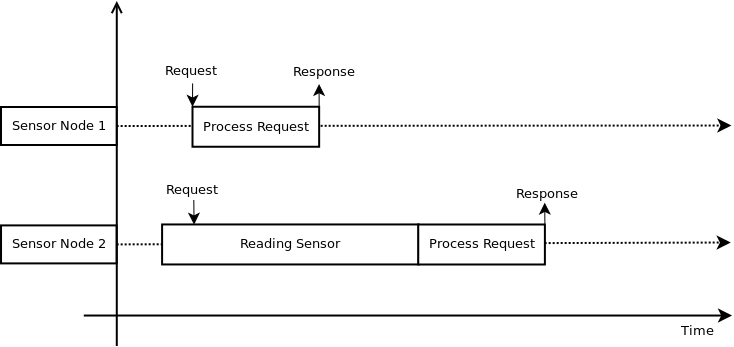
\includegraphics[width=\textwidth]{fig/PingProbe_Theory.png}
	\caption{Variations in Response Time\label{FingerprintTheory}}
\end{figure}

In real life, most sensors are programmed in a loop; therefore the same code fragments are repeated through the life time of a sensor. Each code fragment takes different time to execute and hence the response times vary. This behaviour could be statistically analysed and the resulting distribution could be stored as a `fingerprint' .


For this fingerprinting scenario, we must assume the adversary has the pre-knowledge of potential programs and can fingerprint them (or that they have access to a database that contains this information). To identify an unknown program running on target sensor, the adversary collects a new fingerprint and then matches it to available fingerprints. Clearly, to effectively launch the attack, the adversary needs to be able to send the request to a targeted sensor (requests with short predictable processing time are preferable as they induce less noise). 

In practice, the request can be instantiated by several messages defined in the sensor network protocols. PING is exceptionally ideal as it is mandatory in the ICMP standard\cite{rfc4433} and has only negligible computation. Other options but not excluded are Heartbeat in DTLS\cite{rfc6520}, Reset in CoAP\cite{rfc7252}, etc.

\subsubsection{Extracting Fingerprints}
We explored the feasibility of fingerprinting programs on an CC2538 running Contiki OS by using the PING command.

\Cref{ExamplePri} shows an example of captured packets. Contiki MAC\cite{ContikiMAC} sends duplicated PING requests. The response time, which refers to PING Response Interval, PRI, is defined to be the time between a PING response and its last paired request. The highlighted Packets 205 and 203 shows such an example.

\begin{figure}[!h]
	\centering
	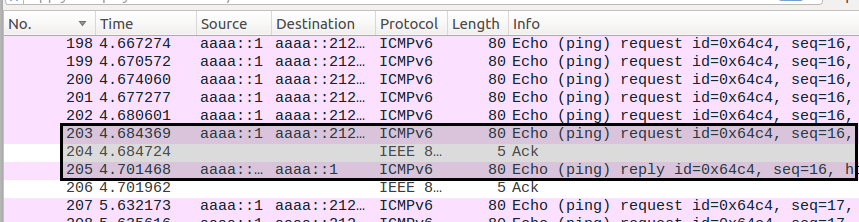
\includegraphics[width=\textwidth]{fig/PRI_hl.png}
	\caption{Example PRI\label{ExamplePri}}
\end{figure}

%Since the attack extracts the information contained in the extended response time of a specific request, the first problem is to see whether such extended response time can be filtered from normal ones. 

\Cref{HelloworldPriNormal} shows the histogram of PRIs collected on the ``helloworld'' example from Contiki OS. Values $\geq$12ms are collected at 12ms. The result shows that most PRIs are clustered around 9.5ms which consists with our result in \Cref{PingResponse}. The majority, roughly ranged [9.0, 10.3]ms, corresponds to the usual response time as depicted by Sensor Node 1 in \Cref{FingerprintTheory}. 

\begin{figure}[!h]
	\centering
	\begin{subfigure}{0.45\textwidth}
		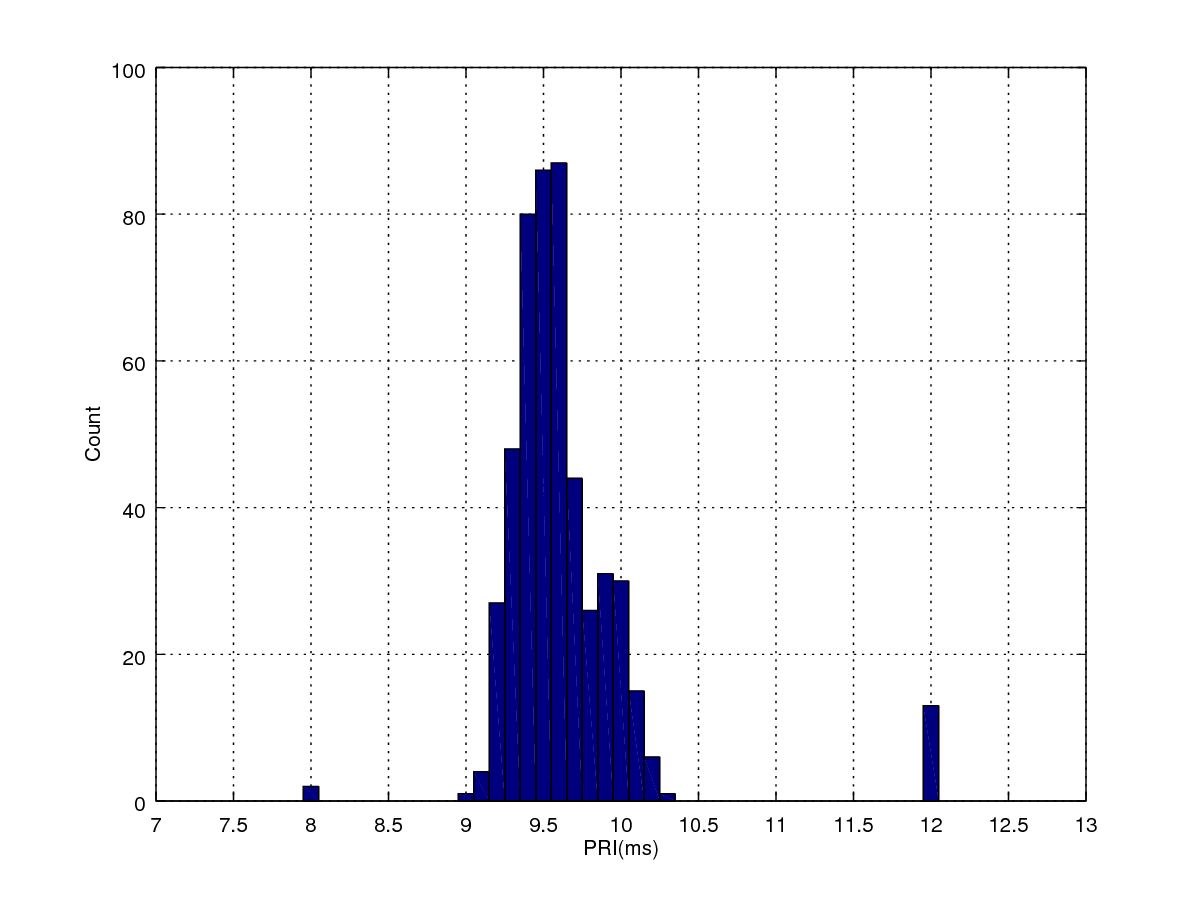
\includegraphics[width=\textwidth]{fig/helloworld_cc2538.png}
		\caption{PRIs of helloworld\label{HelloworldPriNormal}}
	\end{subfigure}
	\begin{subfigure}{0.45\textwidth}
		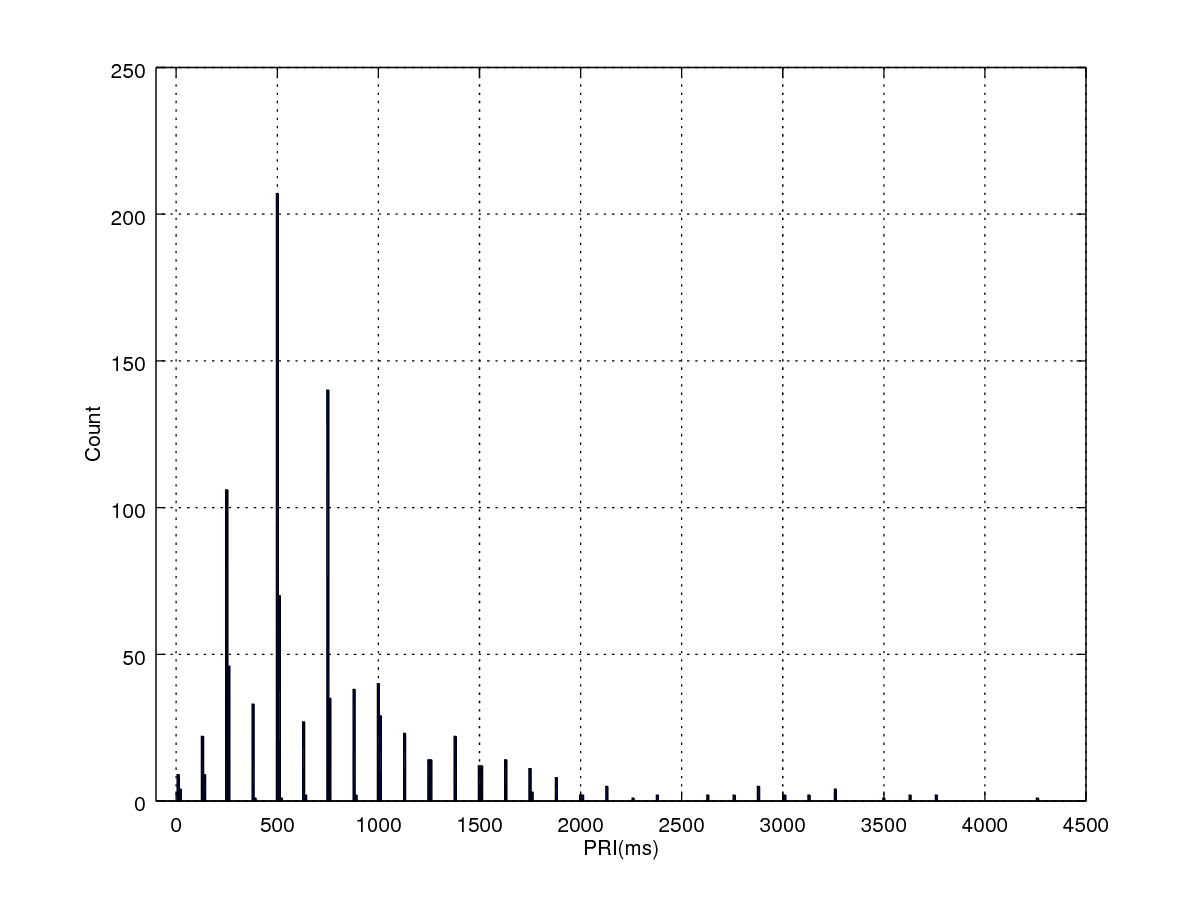
\includegraphics[width=\textwidth]{fig/helloworld_cc2538_outlier.png}
		\caption{PRIs outliers of helloworld\label{HelloworldPriOutliers}}
	\end{subfigure}
	\caption{helloworld PRIs\label{HelloworldPri}}
\end{figure}

We further plotted the upper outliers, mostly ranged [12, 2000]ms, in \Cref{HelloworldPriOutliers}. We suppose these outliers correspond to the extended response time as depicted by Sensor Node 2 in \Cref{FingerprintTheory}. The distribution described by \Cref{HelloworldPriOutliers} is the fingerprint of the ``helloworld'' example.

The result in \Cref{HelloworldPri} shows a clear gap between the usual PRIs and extended PRIs. In fact other applications we experimented also showed the same property. This implies that an adversary can easily draw a threshold by observing the whole PRI distribution and then filter out the fingerprint. In our experiments the threshold is set to 12ms but any other values within the gap would also work. 

We collected the fingerprints for three programs taken from the Contiki OS examples:
\begin{description}
	\item[broadcast] This program periodically broadcasts a constant message.
	 
	\item[powertrace] This program records the power consumption and broadcasts a constant message.
	
	\item[Sensorpayload] This program is based on the ``er-rest-example'' embedded together with sensor accesses taken from ``cc2538-demo''. It captures a real case scenario where three different sensors, namely Temperature, VDD and ALS, are being accessed through CoAP.
\end{description}

Specifically for ``Sensorpayload'' we collected fingerprints for 8 different scenarios where different sensors are being accessed. For each program we independently collected 2 fingerprints for comparison.

\Cref{FingerprintApps} summarises the total 20 fingerprints we collected for the experiment.

\subsubsection{Fingerprint Matching}
%Comparing the distribution.

During the experiments we realised that most of the fingerprints do not adhere to common distributions; therefore we used non parametric test, the Kolmogorov-Smirnov Distance\cite{KsTest}, as our test statistic. \Cref{ksdistances} summarises the relative KS distances computed on each pair of fingerprints in our experiments.

Although fingerprints collected on the same application were rejected by the Kolmogorov-Smirnov Test, we noticed that their KS distance tends to be smaller comparing to fingerprints collected on different programs, as the \textbf{bold} cells marked in \Cref{ksdistances}. 

By adapting our distinguisher to utilise the minimum KS distance, we were able to identify 13 out of 20 fingerprints successfully. The `overlapping' fingerprints are mainly due to the ``Sensorpayload'' program, which access different sensors, but otherwise has identical program code. Thus we did expect that the different instantiations of it would lead to very similar fingerprints. 

\section{Conclusion\label{sec: Conclusion}}

In this paper we explore, for the first time, the use of packet lengths and response times, which are protocol level side channels, as means to recover information about IoT `things'. We do this via some experiments, which we base on two extremely popular devices running on a popular open source OS, with a typical stack of protocols. Whilst we do not cover a wide range of devices, the fact that two of the most popular devices show the characteristics that we hypothesise, gives credibility to our results. Our results show that it is possible (in principle) to recover information about a device and its function (i.e. the hardware and the software that runs on it) via inspecting encrypted traffic that it produces. We also point out that ICMP messages can be distinguished from each other despite the use of encryption. 

In order to mitigate the leakage that is given by packet lengths, previous works recommends padding \cite{Peekaboo}. We echo this recommendation. Whilst padding to MTU is considered inefficient for the Internet, it is in fact highly appropriate for 6LoWPAN because:
\begin{itemize}
	\item It completely hides the length of original plaintext.
	\item 6LoWPAN has only a low MTU of 127 bytes; therefore the overhead is acceptable.
	\item It induces negligible computational overhead.
\end{itemize}

%Resourceful applications can enhance the countermeasure by inserting dummy packets.

With regard to the leaking information about the device or OS, we suggest strictly applying the standard MTU to eliminate the differences in drivers. Although there is a potential of performance downgrade, but it will also improve the compatibility among different devices.


%Two options:
%\begin{itemize}
%	\item Randomise response time: needs to be resilient to statistical analysis.
%	\item Threashold response time (discard or reply in a constant time): performance tradeoff. Recommended for unreliable transmissions.
%\end{itemize}
In order to mitigate the leakage given by response times, the natural countermeasure is to write time-constant code, which is known to be notoriously difficult. But two approaches are available to a software developer:
\begin{itemize}
	\item Randomly delay the response. This essentially adds noise to the measurements of the adversary.
	 
	\item Use a threshold response time, i.e. a request is either responded at a predefined time or not responded at all. 
\end{itemize}
Within the context of 6LoWPAN the second method is recommended as most 6LoWPAN application would tolerate missing packets and timer is available on most platforms. However, the threshold must be carefully chosen to preserve the functionality of the 6LoWPAN application.





\appendix
\section{Fingerprint Experiment Programs}

\begin{table}[!ht]
\center
\begin{tabular}{|c|c|c|c|c|}
\hline
\textbf{Trace Index} & \textbf{Application} & \textbf{Size} & \textbf{Filtered Size} & \textbf{Note}              \\ \hline
1                    & broadcast            & 6489          & 593                    &                            \\ \hline
2                    & broadcast            & 6164          & 639                    &                            \\ \hline
3                    & powertrace           & 7142          & 539                    &                            \\ \hline
4                    & powertrace           & 7079          & 561                    &                            \\ \hline
5                    & Sensorpayload        & 7338          & 987                    & Temperature + Light        \\ \hline
6                    & Sensorpayload        & 7963          & 934                    & Temperature + Light        \\ \hline
7                    & Sensorpayload        & 7143          & 1195                   & Temperature only           \\ \hline
8                    & Sensorpayload        & 7316          & 1096                   & Temperature only           \\ \hline
9                    & Sensorpayload        & 7895          & 827                    & Light only                 \\ \hline
10                   & Sensorpayload        & 7867          & 789                    & Light only                 \\ \hline
11                   & Sensorpayload        & 7428          & 1138                   & No reading                 \\ \hline
12                   & Sensorpayload        & 7462          & 833                    & No reading                 \\ \hline
13                   & Sensorpayload        & 6565          & 1391                   & VDD only                   \\ \hline
14                   & Sensorpayload        & 7193          & 1111                   & VDD only                   \\ \hline
15                   & Sensorpayload        & 7672          & 955                    & Temperature, Light and VDD \\ \hline
16                   & Sensorpayload        & 7790          & 1023                   & Temperature, Light and VDD \\ \hline
17                   & Sensorpayload        & 7864          & 931                    & Light + VDD                \\ \hline
18                   & Sensorpayload        & 7936          & 987                    & Light + VDD                \\ \hline
19                   & Sensorpayload        & 7217          & 1222                   & Temperature + VDD          \\ \hline
20                   & Sensorpayload        & 7050          & 1228                   & Temperature + VDD          \\ \hline
\end{tabular}
\caption{PingProbe Experiment Applications}
\label{PingProbeApps}
\end{table}


\section{Fingerprint Experiment Relative KS-Distances}

\begin{sidewaystable}[!ht]
\footnotesize
\begin{center}
\begin{tabular}{|c|c|c|c|c|c|c|c|c|c|c|c|c|c|c|c|c|c|c|c|c|}
\hline
Index & 1 & 2 & 3 & 4 & 5 & 6 & 7 & 8 & 9 & 10 & 11 & 12 & 13 & 14 & 15 & 16 & 17 & 18 & 19 & 20 \\ \hline
1 & N/A & \textbf{7.8} & 75 & 78.9 & 48.3 & 58.4 & 19.2 & 15.8 & 62.2 & 58.5 & 34.2 & 34 & 13.2 & 10.3 & 54.1 & 57 & 52.8 & 58.7 & 19.4 & 13.3 \\ \hline
2 & \textbf{7.8} & N/A & 81.7 & 85.6 & 54.8 & 65.1 & 25.6 & 22.4 & 68.7 & 65 & 40.8 & 40.4 & 14.9 & 16.7 & 60.7 & 63.7 & 59.3 & 65.4 & 26 & 19.3 \\ \hline
3 & 75 & 81.7 & N/A & \textbf{6.9} & 30.3 & 22.9 & 56.3 & 59.5 & 16.2 & 21.2 & 41.2 & 41.5 & 67 & 65 & 21.5 & 22.8 & 23.2 & 29.8 & 55.8 & 62.5 \\ \hline
4 & 78.9 & 85.6 & \textbf{6.9} & N/A & 32.3 & 22.5 & 60.3 & 63.6 & 17.9 & 20.9 & 45.2 & 45.6 & 71 & 69.3 & 25.2 & 22.5 & 26.7 & 27.4 & 59.8 & 66.7 \\ \hline
5 & 48.3 & 54.8 & 30.3 & 32.3 & N/A & \textbf{11.3} & 29.4 & 32.7 & 15.1 & 14 & 14.5 & 14.7 & 40.1 & 38.3 & 14.8 & 16.1 & 17.1 & 23.8 & 28.9 & 35.6 \\ \hline
6 & 58.4 & 65.1 & 22.9 & 22.5 & 11.3 & N/A & 39.5 & 42.9 & 9 & \textbf{4.9} & 24.4 & 24.7 & 50.3 & 48.4 & 14 & 16 & 16.8 & 23.7 & 39.2 & 45.8 \\ \hline
7 & 19.2 & 25.6 & 56.3 & 60.3 & 29.4 & 39.5 & N/A & \textbf{4.4} & 43.2 & 39.5 & 19.7 & 17 & 14.5 & 9.6 & 35.3 & 38.5 & 33.7 & 39.7 & 10.8 & 9.6 \\ \hline
8 & 15.8 & 22.4 & 59.5 & 63.6 & 32.7 & 42.9 & \textbf{4.4} & N/A & 46.6 & 42.8 & 19.5 & 19.1 & 14.9 & 6.2 & 38.4 & 41.7 & 37.1 & 43.2 & 10.9 & 9 \\ \hline
9 & 62.2 & 68.7 & 16.2 & 17.9 & 15.1 & 9 & 43.2 & 46.6 & N/A & \textbf{5.4} & 28.2 & 29 & 54 & 52.1 & 10.3 & 12.4 & 12.3 & 19 & 42.8 & 49.7 \\ \hline
10 & 58.5 & 65 & 21.2 & 20.9 & 14 & \textbf{4.9} & 39.5 & 42.8 & 5.4 & N/A & 24.5 & 25.4 & 50.2 & 48.4 & 11.5 & 13.4 & 14.4 & 20.9 & 39.1 & 46.4 \\ \hline
11 & 34.2 & 40.8 & 41.2 & 45.2 & 14.5 & 24.4 & 19.7 & 19.5 & 28.2 & 24.5 & N/A & \textbf{7.4} & 28.2 & 24.7 & 20 & 23.1 & 19 & 24.7 & 15 & 23.9 \\ \hline
12 & 34 & 40.4 & 41.5 & 45.6 & 14.7 & 24.7 & 17 & 19.1 & 29 & 25.4 & \textbf{7.4} & N/A & 25.7 & 23.9 & 20.7 & 23.7 & 19 & 25 & 14.9 & 21.7 \\ \hline
13 & 13.2 & 14.9 & 67 & 71 & 40.1 & 50.3 & 14.5 & 14.9 & 54 & 50.2 & 28.2 & 25.7 & N/A & 11.7 & 45.9 & 49.2 & 44.5 & 50.6 & 15.7 & \textbf{8.9} \\ \hline
14 & 10.3 & 16.7 & 65 & 69.3 & 38.3 & 48.4 & 9.6 & \textbf{6.2} & 52.1 & 48.4 & 24.7 & 23.9 & 11.7 & N/A & 44 & 47.2 & 42.8 & 48.7 & 10.5 & 7.2 \\ \hline
15 & 54.1 & 60.7 & 21.5 & 25.2 & 14.8 & 14 & 35.3 & 38.4 & 10.3 & 11.5 & 20 & 20.7 & 45.9 & 44 & N/A & \textbf{3.8} & 6.7 & 11.2 & 34.8 & 41.5 \\ \hline
16 & 57 & 63.7 & 22.8 & 22.5 & 16.1 & 16 & 38.5 & 41.7 & 12.4 & 13.4 & 23.1 & 23.7 & 49.2 & 47.2 & \textbf{3.8} & N/A & 8.8 & 8.9 & 37.9 & 44.7 \\ \hline
17 & 52.8 & 59.3 & 23.2 & 26.7 & 17.1 & 16.8 & 33.7 & 37.1 & 12.3 & 14.4 & 19 & 19 & 44.5 & 42.8 & \textbf{6.7} & 8.8 & N/A & 11.5 & 33.6 & 40 \\ \hline
18 & 58.7 & 65.4 & 29.8 & 27.4 & 23.8 & 23.7 & 39.7 & 43.2 & 19 & 20.9 & 24.7 & 25 & 50.6 & 48.7 & 11.2 & \textbf{8.9} & 11.5 & N/A & 39.4 & 46.1 \\ \hline
19 & 19.4 & 26 & 55.8 & 59.8 & 28.9 & 39.2 & 10.8 & 10.9 & 42.8 & 39.1 & 15 & 14.9 & 15.7 & 10.5 & 34.8 & 37.9 & 33.6 & 39.4 & N/A & \textbf{10.3} \\ \hline
20 & 13.3 & 19.3 & 62.5 & 66.7 & 35.6 & 45.8 & 9.6 & 9 & 49.7 & 46.4 & 23.9 & 21.7 & 8.9 & \textbf{7.2} & 41.5 & 44.7 & 40 & 46.1 & 10.3 & N/A \\ \hline
\end{tabular}
\end{center}
\caption{
KS Distances of PingProbe Experiment Traces (multiplied by 100 for readability).
Minimum in each row marked as \textbf{bold}.
}
\label{ksdistances}
\end{sidewaystable}

%And this is my Appendix.

%\subsection*{Appendix Subsection}

%Some text.

%\nocite{*} % add all entries from sample.bib

\bibliography{references,rfc}
%\begin{thebibliography}{10}



%\end{thebibliography}

%\section*{Biography}
%
%\fbox{\parbox[t]{3cm}{Here is space for \\
%a photograph of \\
%the author. \\
%\vspace*{2cm}
%}}
%
%\medskip
%\noindent
%{\bf Author's name}. A short vitae can be included here.

\end{document}
